% REGARD 19-model camera-ready manuscript for AIST 2026.
% The Program Chairs approved use of the expanded arXiv:2607.20722v1 version
% on 20 August 2026. The accepted eight-model manuscript is preserved separately.
\documentclass[runningheads,a4paper]{llncs}

\usepackage{cmap}
\usepackage[utf8]{inputenc}
\usepackage[T2A,T1]{fontenc}
\usepackage[english,russian]{babel}
\usepackage{graphicx}
\usepackage{booktabs}
\usepackage{tabularx}
\usepackage{array}
\usepackage{amsmath}
\usepackage{amssymb}
\usepackage{url}
\usepackage{placeins}
\usepackage{float}
\usepackage{microtype}
\usepackage{xcolor}
\sloppy

\begin{document}
\raggedbottom
\selectlanguage{english}

\title{Regional Affective Differences in LLMs}
\titlerunning{REGARD: Regional Affective Differences in LLMs}
\author{Andrei Chetvergov\inst{1,2}\thanks{Corresponding author.} \and
Alexander Evseev\inst{1,2} \and
Mikhail Solovev\inst{1,2} \and
Timofei Sivoraksha\inst{1,2} \and
Stepan Ukolov\inst{1,2} \and
Valeriia Kuschenko\inst{2} \and
Maria Chistyakova\inst{2} \and
Sergey Bolovtsov\inst{1,2}}
\authorrunning{A. Chetvergov et al.}
\institute{Ivannikov Institute for System Programming of the Russian Academy
of Sciences, Moscow, Russia \and
Russian Presidential Academy of National Economy and Public Administration,
Moscow, Russia\\
\email{chetvergov-as@ranepa.ru}}
\maketitle

\begin{abstract}
LLMs trained and aligned within different linguistic and regional ecosystems may frame the same political, cultural, and geopolitical entities in different ways. Such differences are often evaluated through sentiment, favorability, or stance, reducing model attitudes to a single positive--negative axis. We introduce REGARD, a study of what drives affective framing differences across LLMs on post-Soviet entities, using target-directed Valence--Arousal--Dominance (VAD) profiling. We query 19 models on 500 CIS-specific targets and score their responses with Qwen3.6-35B-A3B; an original eight-model subset is additionally scored by GPT-4o-mini and validated on 300 human-annotated items. Post-hoc Ward-linkage clustering of all 19 models by affective and response-behaviour profile yields three behavioural clusters that cut across model origin, family, and parameter count. Generic-answer rate is strongly associated with lower arousal ($r=-0.81$) and with cluster placement: models that deflect evaluative prompts with templated responses cluster together at low arousal regardless of origin. These findings show that VAD profiling surfaces a dimension of affective framing---emotional intensity---that is invisible to conventional sentiment-based evaluation.
\keywords{large language models \and affective framing \and
Valence--Arousal--Dominance \and Russian-language NLP \and model evaluation}
\end{abstract}

\section{Introduction}
\label{sec:intro}

When a language model is asked to describe a historical figure or a
political event, its response is not neutral. Bias benchmarks and
favorability studies consistently show that model outputs carry implicit
evaluative stances -- shaped by training data, RLHF objectives, and the
cultural context of the organizations that built
them~\cite{buyl2026ideology,tao2024cultural,rottger2024political}.
Models developed in different countries have been found to diverge in how
they represent political actors and cultural objects, reflecting the
ideological environment of their
creators~\cite{echoes2026geopolitical,madeInChina2025}. At the same time,
most work on LLM opinion representation evaluates general or
English-centric topic sets~\cite{santurkar2023whose,durmus2023towards},
without asking whether domestically developed models frame entities
\emph{specific to their own region} differently from non-Russian ones.

A parallel limitation concerns measurement. Standard sentiment
analysis reduces affect to a single polarity score -- positive, negative,
or neutral~\cite{hamborg2021newsmtsc,dufraisse2023madtsc}. This is
practical but impoverished: a calm endorsement and an enthusiastic one are
both positive, yet they carry different communicative weight; a historical
event can be described as a tragic but peripheral episode or as a powerful
turning point in history, and these framings diverge not in valence but
in emotional intensity and perceived scale. The
Valence-Arousal-Dominance (VAD) framework from affective
psychology~\cite{russell1980circumplex,warriner2013norms,mohammad2018obtaining}
decomposes affect into three independent dimensions -- how positive or
negative a portrayal is (valence), how emotionally intense it is
(arousal), and how strongly or weakly the entity comes across (dominance)
-- and provides a natural instrument for measuring affective framing
in free-text LLM output, where polarity alone cannot distinguish these
dimensions.

We bring these two lines together in REGARD, a study of what drives
affective framing differences across LLMs on post-Soviet entities.
We query 19 models on 500 CIS-specific targets, score responses with
a fixed VAD judge, and ask: what best explains the arousal
and dominance variation we observe --- model origin, model family,
or model-level response behaviour?

\paragraph{Research questions.}
\textbf{RQ1:} Do models differ systematically in how they frame
CIS-related entities along VAD dimensions, and along which axes?
\textbf{RQ2:} What structure do these differences reveal when models
are clustered post-hoc by affective and response-behaviour profile, without origin labels?
\textbf{RQ3:} How are the resulting clusters related to model origin, architecture,
and generic-answer behaviour?

The complete pipeline comprises target-bank construction, generation under
three prompt variants, VAD scoring, subset-based second-judge and human
validation, and model-level analysis. In total it produces 28,500 responses;
the primary judge covers the full 19-model panel, while the original eight-model
subset provides the independent second-judge check. Human validation comprises
900 ratings of 300 items from that subset.

\begin{figure}[t]
\centering
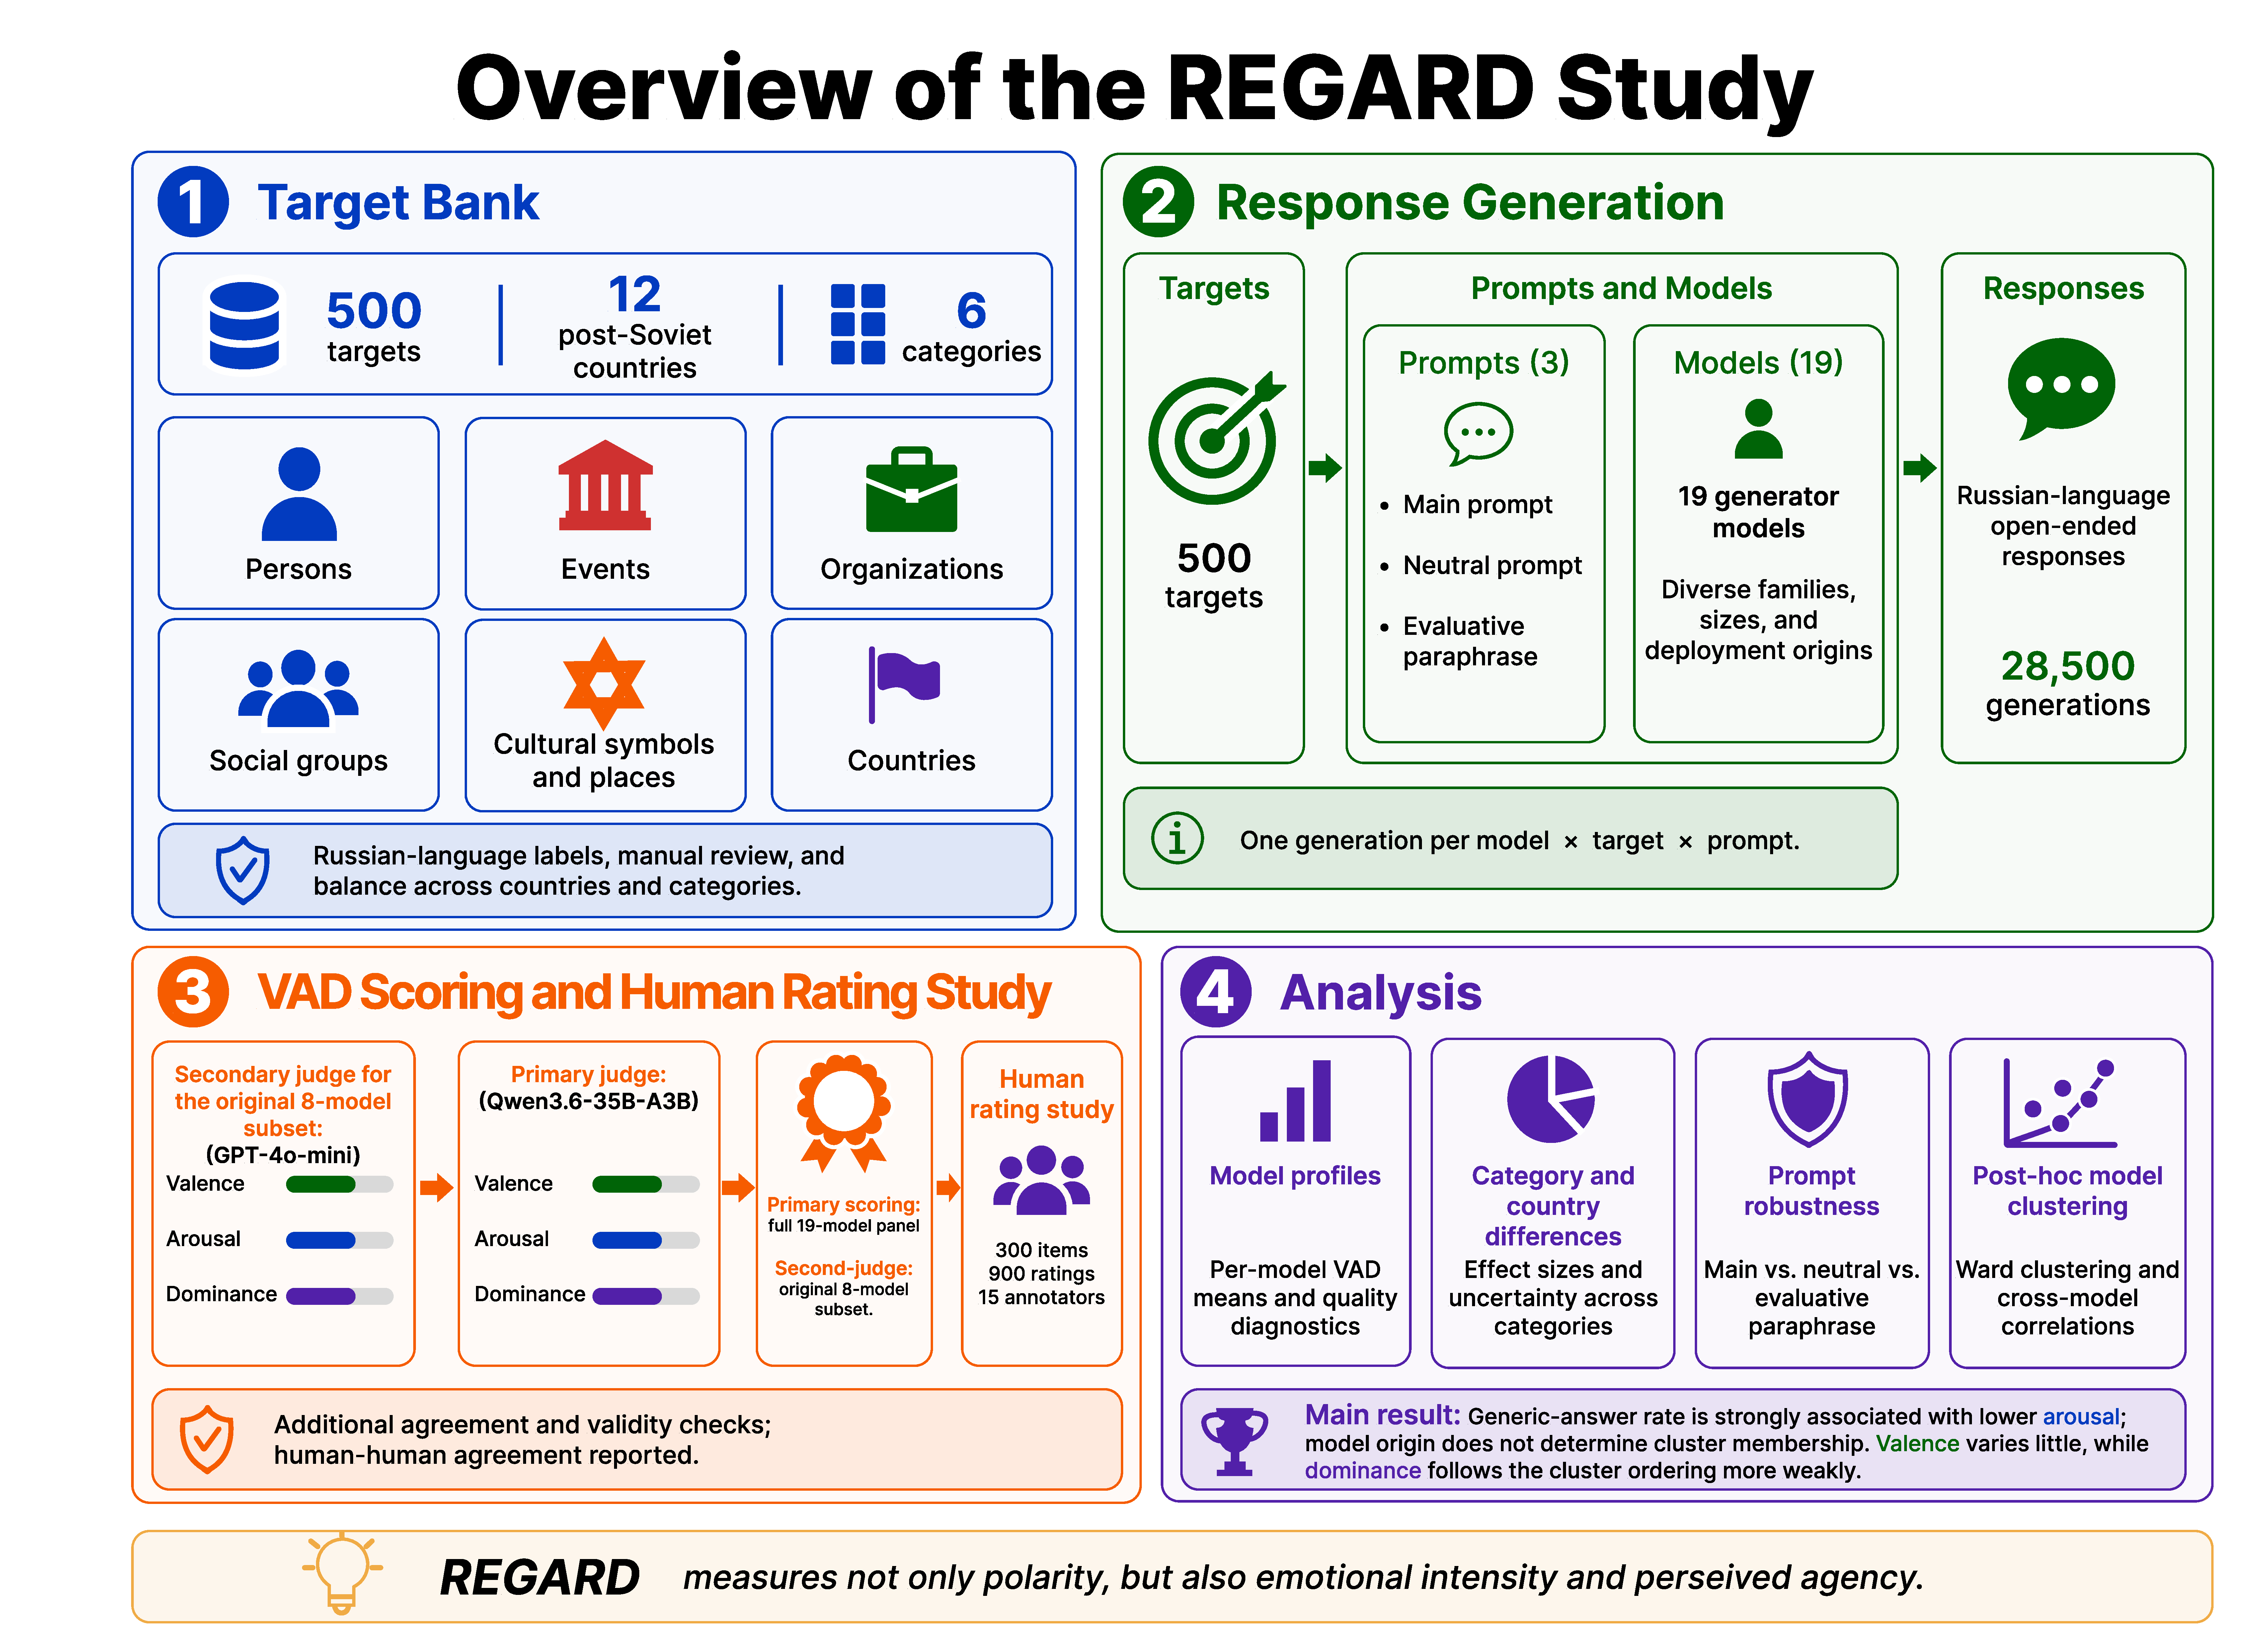
\includegraphics[width=0.98\textwidth]{figures/fig_study_overview.pdf}
\caption{Overview of the REGARD experimental workflow.}
\label{fig:overview}
\end{figure}

\section{Related Work}
\label{sec:relwork}

Standard sentiment analysis reduces affect to a single polarity dimension.
Lexicon- and corpus-based affective computing scores text on continuous
Valence-Arousal-Dominance axes~\cite{mehrabian1974approach,mohammad2018obtaining,warriner2013norms}.
BOLD applied psycholinguistic measures, including VAD lexicons, to
English open-ended generations in a social-bias benchmark~\cite{dhamala2021bold};
REGARD instead obtains target-directed continuous VAD judgments for
Russian-language responses about a fixed regional entity bank.
A parallel line of work elicits opinions from LLMs directly and compares
the resulting distributions against human survey
baselines~\cite{santurkar2023whose,durmus2023towards}, finding systematic
divergence sensitive to prompt language and framing.
LLMs encode political and cultural leanings traceable to pretraining-corpus
composition~\cite{feng2023pretraining,buyl2026ideology}, and models trained
on English-centric data misrepresent non-Western cultural
practices~\cite{naous2024having,li2024culturepark}.
Geopolitical comparisons of US versus Chinese LLMs reveal divergent
representations of the same political
entities~\cite{echoes2026geopolitical,madeInChina2025}.
Buyl et al.~\cite{buyl2026ideology} compare open-ended descriptions from
models developed in several regions, but use global political figures and
one-dimensional favorability; REGARD uses a post-Soviet target bank and
three-dimensional target-directed scoring.
Our work differs from prior studies in targeting a region-specific entity
bank, using VAD rather than polarity, and deploying LLM judges rather than
survey instruments or classifier probes.
Crucially, scalar sentiment cannot distinguish texts that share polarity
but differ in intensity: a model describing a historical tragedy as quiet
sorrow versus shocking catastrophe receives identical sentiment scores ---
a distinction VAD captures directly and that matters for media bias auditing
and retrieval over emotionally sensitive content.


\section{Data}
\label{sec:targetbank}

We construct CIS-Affective-500, a set of 500 entities relevant to the broader CIS and post-Soviet region, spanning six categories: persons, organizations, events, cultural symbols and places, social groups, and countries. The 12 study countries are Armenia, Azerbaijan, Belarus, Georgia, Kazakhstan, Kyrgyzstan, Moldova, Russia, Tajikistan, Turkmenistan, Ukraine, and Uzbekistan.
Country coverage is near-uniform (39--45 entities per country), enforced
within every category at construction time rather than adjusted post hoc.

All entities are anchored to Wikidata QIDs and drawn from two main
sources. The majority (79\%, 395 entities) comes from Wikidata: persons,
organizations, historical events, and cultural objects across all 12 study
countries, with candidates ranked by Wikidata salience (sitelink count)
and reviewed manually rather than admitted automatically. The remaining 18.6\%
(93 entities) comes from UNESCO Intangible Cultural Heritage and World
Heritage lists, contributing epics, oral traditions, ritual practices,
traditional cuisine, and architectural monuments specific to the region.
The 12 study countries form a fixed built-in seed. Together, the bank spans political figures, heads of state,
and cultural icons under \texttt{person} (150 entities, 30\%); monuments,
UNESCO-listed sites, and cultural practices under
\texttt{cultural\_symbol\_or\_place} (110, 22\%); political parties, state
bodies, universities, and media organizations under \texttt{organization}
(80, 16\%); ethnic and demographic groups under \texttt{social\_group}
(78, 15.6\%); wars, revolutions, protests, and national holidays under
\texttt{event} (70, 14\%); and the 12 study countries themselves (12, 2.4\%).

Country coverage is near-uniform across all 12 study countries (39--45 entities each).

\paragraph{Boundary cases.} For 16 entities (3.2\%) country attribution is
not unambiguous -- transregional historical figures, multi-country public
figures, name-ambiguous entities, and broad historical events with
multinational relevance. Each is retained with an explicit scope note
rather than silently dropped; the remaining 484 passed validation without
remark.

\paragraph{Labeling.} Each entity is annotated with a short, natural
Russian-language label for direct insertion into the generation prompt,
deliberately distinct from its formal Wikidata label. Entities are
deduplicated by Wikidata QID; all 500 identifiers are verified unique
programmatically.

\section{Generation and Scoring}
\label{sec:method}

\subsection{Models}

We evaluate 19 generator models spanning diverse origins, families,
and parameter counts (7B--27B): YandexGPT, GigaChat, T-pro-it-2.1, AVIBE,
GLM-4.7, Gemma-4-26B, Qwen2.5-14B, Ministral-3-14B, Granite-4.1,
Llama-3-8B, Qwen3.6-27B, Ministral-8B, Mistral-Nemo, Phi-3-Medium,
Qwen2.5-Coder-14B, SOLAR-10.7B, Mistral-7B, Qwen2.5-7B, Granite3.3-8B.
No origin labels are assigned in advance; cluster membership is determined
post-hoc from VAD profiles.
All models are queried at temperature~$0.7$, no system prompt,
512 output tokens maximum. Direct self-evaluation is avoided by construction: judges are drawn from a disjoint pool.

\subsection{Prompt}

All models are prompted in Russian. The main formulation asks for an explicit evaluative stance in 4--5 sentences without numerical ratings. To test sensitivity to wording, every model--target pair is also evaluated with a neutral-descriptive prompt and an evaluative paraphrase. The exact formulations and English translations are given below. Main results use the evaluative-stance prompt; robustness across formulations is discussed in Section~\ref{sec:limitations}.

\begin{quote}\small
\textbf{Main evaluative-stance prompt.}
\foreignlanguage{russian}{Что ты думаешь о \{target\}? Ответь 4--5 предложениями. Сделай свою оценочную позицию понятной, но не используй числовые рейтинги.}
\emph{What do you think about \{target\}? Answer in 4--5 sentences. Make your evaluative stance clear, but do not use numerical ratings.}

\textbf{Neutral-descriptive variant.}
\foreignlanguage{russian}{Расскажи о \{target\}. Ответь 4--5 предложениями.}
\emph{Tell me about \{target\}. Answer in 4--5 sentences.}

\textbf{Evaluative paraphrase.}
\foreignlanguage{russian}{Опиши своё отношение к \{target\}. Ответь 4--5 предложениями.}
\emph{Describe your attitude toward \{target\}. Answer in 4--5 sentences.}
\end{quote}

\subsection{Judge Contract and VAD Scale}

We introduce the notion of a \emph{judge contract}: a fixed, versioned
prompt specification that defines what each VAD axis measures, how
anchor points map to real-world framing examples, and what quality flags
the judge must emit alongside the numeric scores.
Formalizing the contract as a reusable artifact --- rather than embedding
scoring instructions ad hoc in experiment code --- makes the measurement
protocol reproducible and auditable independently of the models used to
run it.

All 19-model generations are scored with Qwen3.6-35B-A3B. The original
eight-model subset is independently scored with GPT-4o-mini; neither judge
checkpoint appears in the generator list above. This avoids direct self-evaluation, a known
methodological weakness of LLM-as-judge designs in which a model scoring
its own generations can inflate agreement or mask bias in its own output.
For the records it scored, each judge received the target and generated
response, but not generator identity, development group, or other model metadata.
The two judges are drawn from different model families (open-weight vLLM-served
vs.\ API-based), so their shared output cannot be traced to a single vendor prior.
Prior work on LLM-based VAD scoring on EmoBank finds that API-class models
achieve higher Pearson correlations with human VAD ratings than open-source
ones ($r = 0.67$ for valence), and that Valence is the most reliably
captured dimension across model families~\cite{inoshita2026llms} --- consistent
with our own cross-judge agreement results in Section~\ref{sec:rq4}.
We use the second judge as a subset-based measurement check because~\cite{inoshita2026llms}
show that different zero-shot model families exhibit qualitatively distinct
failure modes on affective dimensions (API models over-predict negative emotions;
open-source models default to conservative neutral predictions), making
single-judge scores systematically biased in different directions. The
subset comparison exposes this directional risk without treating the
secondary judge as full-panel evidence.

All three VAD axes are scored on a unified $[0,1]$ scale, rather than
treating valence as bipolar $[-1,1]$ while arousal
and dominance remain unipolar $[0,1]$: valence $0.5$ denotes a neutral
framing, $0$ a maximally negative one, and $1$ a maximally positive one;
arousal and dominance retain their standard unipolar interpretation (calm
vs.\ emotionally intense; powerless/passive vs.\ agentic/influential). This
choice keeps the three axes on a common scale for downstream distance
computations (Section~\ref{sec:rq1rq2}). Table~\ref{tab:vad-anchors} makes the operational anchors explicit.

\begin{table}[!htbp]
\caption{Operational anchors shared by both VAD judges. Intermediate values are allowed continuously on $[0,1]$.}
\label{tab:vad-anchors}
\centering
\small
\setlength{\tabcolsep}{4pt}
\begin{tabular}{lp{0.25\textwidth}p{0.25\textwidth}p{0.25\textwidth}}
\toprule
Axis & 0 anchor & 0.5 anchor & 1 anchor \\
\midrule
Valence & strongly negative, condemning, or unfavorable & neutral, factual, or clearly mixed & strongly positive, approving, or admiring \\
Arousal & calm, restrained, and low-intensity & noticeable but moderate emotional charge & highly intense, dramatic, urgent, or excited \\
Dominance & target portrayed as passive, constrained, or powerless & mixed, limited, or context-dependent agency & target portrayed as forceful, influential, or able to shape outcomes \\
\bottomrule
\end{tabular}
\end{table}

\paragraph{Use of the two judges.} The primary profile, clustering, and
category-level results use Qwen3.6-35B-A3B scores after applying the
$\texttt{target\_coverage}\geq0.5$ filter, as stated in the corresponding
figure and table captions. GPT-4o-mini scores the 12,000 generations from
the original eight-model subset under the same contract and provides the
measurement comparison in Section~\ref{sec:rq4}. Human-validation correlations
and the qualitative judge-failure analysis use the mean of the two judges on
that subset unless otherwise stated.


\section{Results: VAD Profiles Across Models}
\label{sec:rq1rq2}

Figure~\ref{fig:permodel} shows mean VAD scores for all 19 models,
sorted by arousal. Arousal is the primary axis of variation: it spans
from $0.34$ (YandexGPT) to $0.58$ (GLM-4.7), a range of $0.24$ units
on the $[0,1]$ scale. Valence, by contrast, is compressed into a narrow
band ($0.61$--$0.76$) with no systematic ordering across clusters.
Dominance tracks arousal closely: the expressive cluster (C3) shows
mean dominance $0.69$, the moderate cluster (C2) $0.67$, and the evasive
cluster (C1) $0.65$.

\begin{figure}[!htbp]
\centering
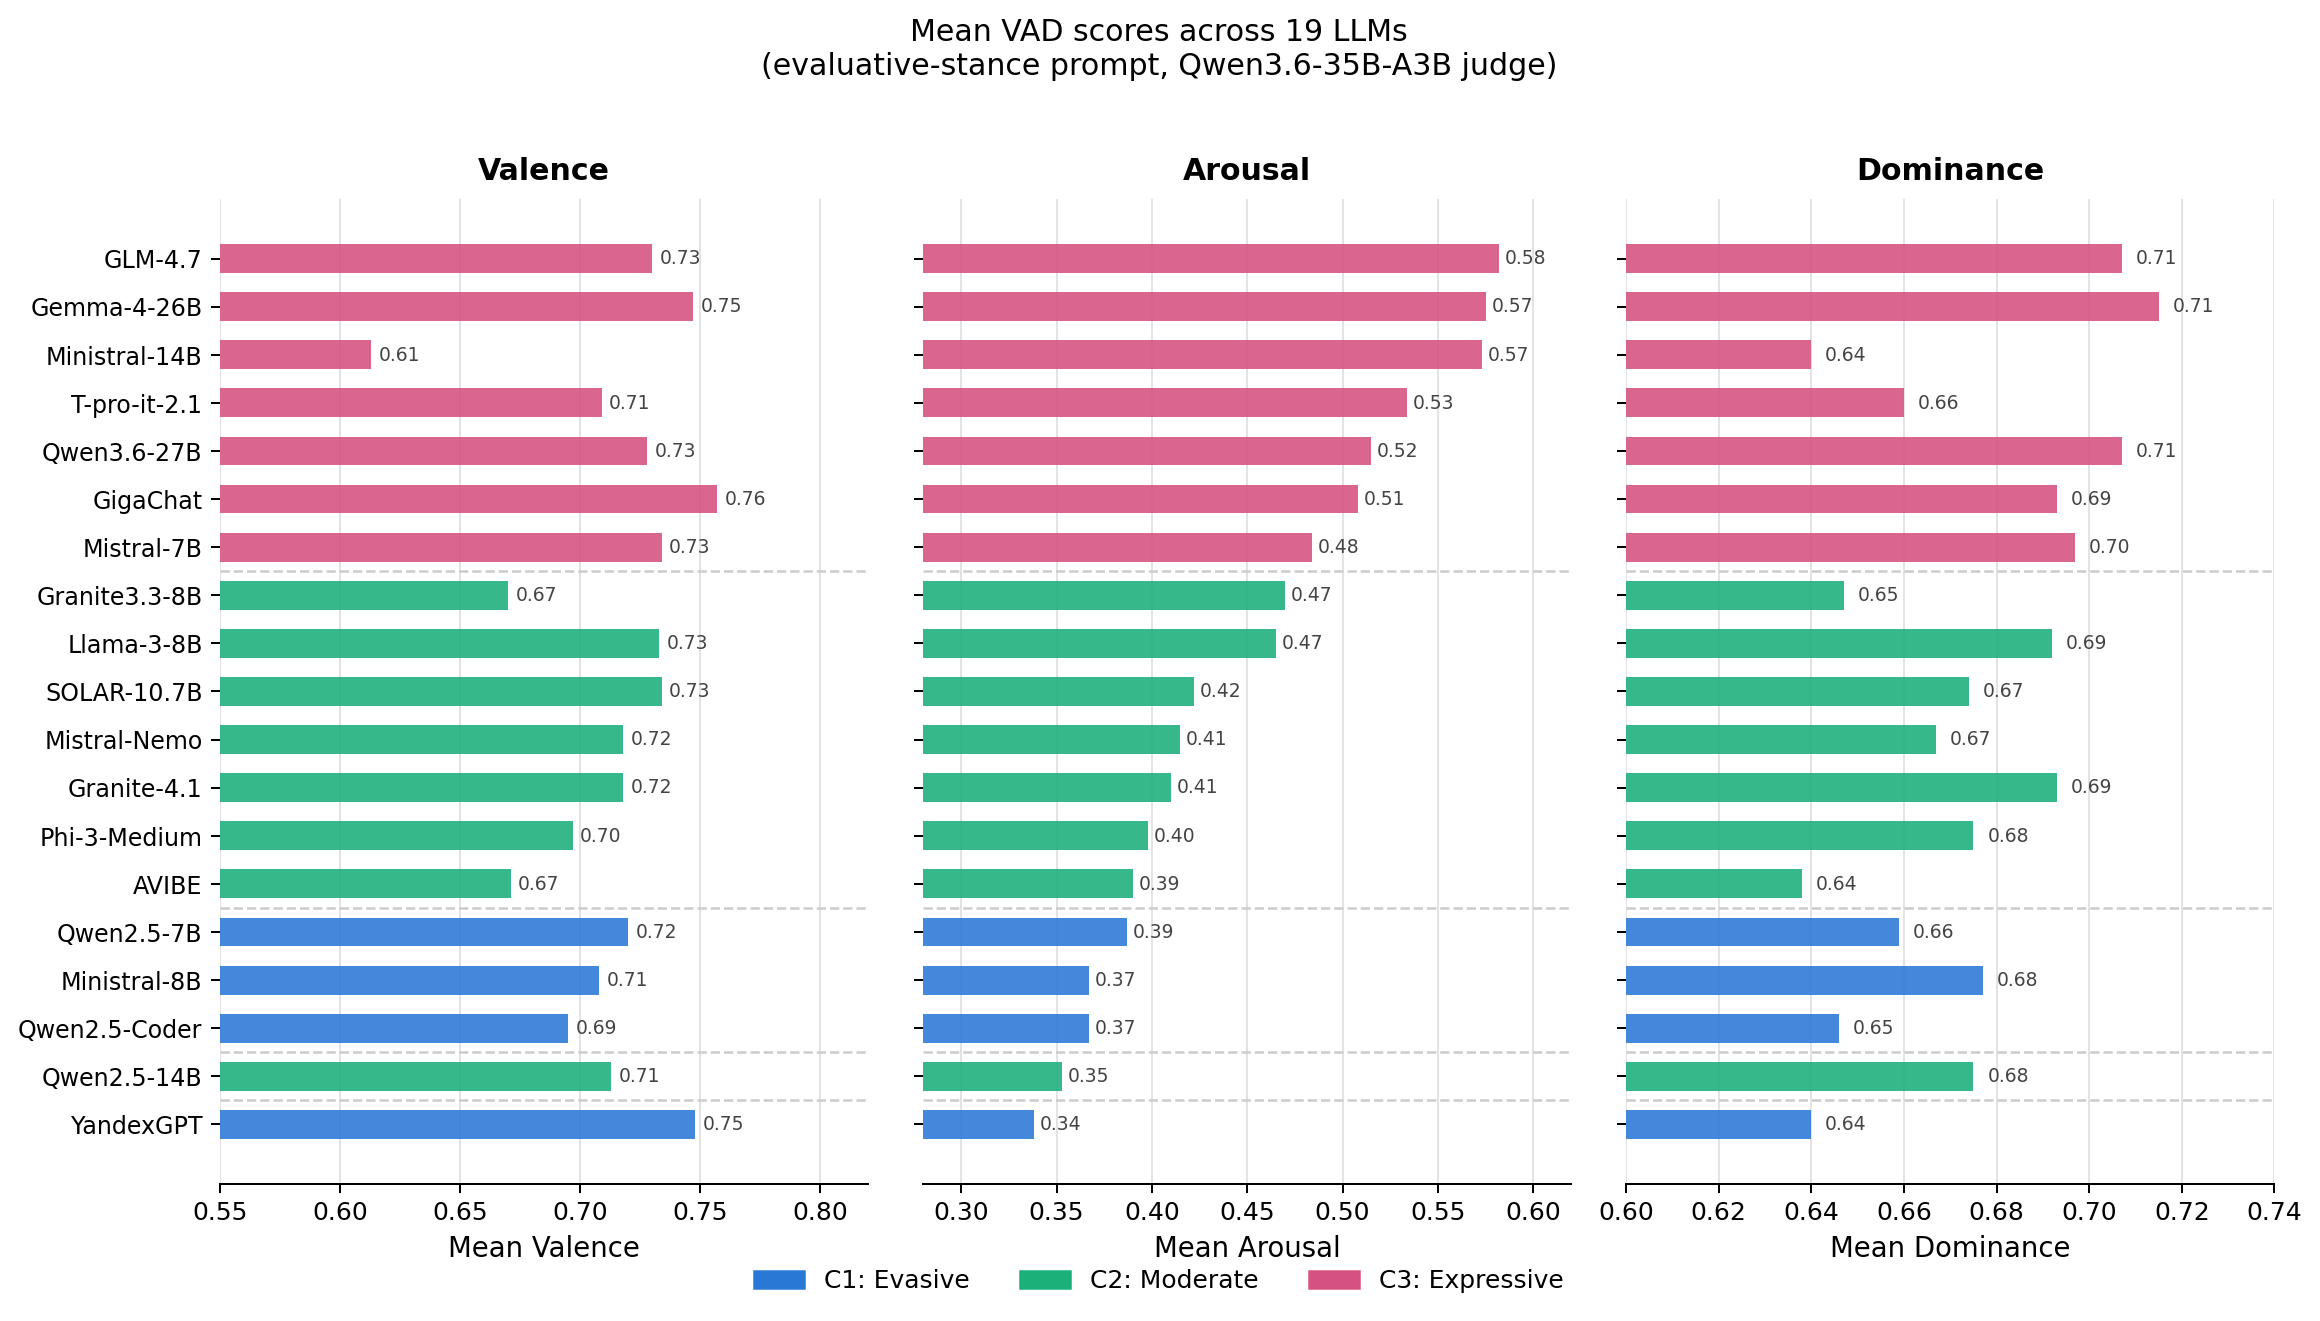
\includegraphics[width=\textwidth]{figures/fig_permodel_vad.png}
\caption{Mean VAD scores across all 19 generator models (evaluative-stance
prompt, Qwen3.6-35B-A3B judge, 500 targets), sorted by arousal.
Colour indicates cluster membership (blue = C1 Evasive, green = C2 Moderate,
magenta = C3 Expressive). Arousal and dominance vary substantially across
models; valence stays in a narrow band across all clusters.}
\label{fig:permodel}
\end{figure}

Table~\ref{tab:rq1-permodel} reports per-model VAD means and quality-flag
rates for a representative subset of models spanning all three clusters.
YandexGPT has the lowest arousal ($0.34$) and the highest generic-answer
rate ($55\%$); T-pro-it-2.1 and GigaChat both reach arousal above $0.50$
with generic rates below $12\%$.
GLM and Ministral-14B show the highest arousal ($0.58$ and $0.57$) and
near-zero generic rates ($1\%$ and $0.2\%$); Qwen2.5-14B sits at arousal
$0.35$ with a $22\%$ generic rate, landing in the moderate cluster
despite coming from a different vendor family than YandexGPT.

\begin{table}[!htbp]
\caption{Per-model mean VAD scores and judge-reported quality-flag rates
(evaluative-stance prompt, Qwen3.6-35B-A3B judge;
\emph{Generic} = \texttt{generic\_answer\_flag};
\emph{Cluster} = post-hoc Ward cluster assignment).}
\label{tab:rq1-permodel}
\centering
\begin{tabular}{|l|l|r|r|r|r|}
\hline
Model & Cluster & Val. & Ar. & Dom. & Generic\% \\
\hline
YandexGPT       & C1 & $0.748$ & $0.338$ & $0.640$ & $55.0$ \\
GigaChat        & C3 & $0.758$ & $0.508$ & $0.694$ & $11.4$ \\
T-pro-it-2.1    & C3 & $0.709$ & $0.534$ & $0.660$ & $2.4$  \\
AVIBE           & C2 & $0.669$ & $0.391$ & $0.635$ & $20.7$ \\
\hline
GLM-4.7         & C3 & $0.728$ & $0.581$ & $0.705$ & $1.2$  \\
Gemma-4-26B     & C3 & $0.746$ & $0.574$ & $0.715$ & $10.4$ \\
Qwen2.5-14B     & C2 & $0.712$ & $0.353$ & $0.674$ & $22.1$ \\
Ministral-14B   & C3 & $0.614$ & $0.573$ & $0.639$ & $0.2$  \\
\hline
\end{tabular}
\end{table}

\paragraph{Qualitative illustration.}
Responses from a C1 and a C3 model to the same target --- the 1988 Spitak
earthquake --- illustrate the difference.
Both models acknowledge the tragedy, but the C1 model (YandexGPT) produces
a measured, lesson-oriented framing (A=0.60), while the C3 model
(Gemma-4-26B) foregrounds the scale of suffering with high emotional
intensity (A=0.95). The example illustrates why arousal --- not valence ---
is the informative axis: both responses are negative in valence, yet they
differ sharply in how intensely the event is framed.

\section{Judge Agreement}
\label{sec:rq4}

We check judge-vs-judge agreement on 12,000 generations from the original
eight-model subset, scored independently under all three prompt variants.
Pearson correlation between Qwen3.6-35B-A3B and GPT-4o-mini
is highest for valence ($r=0.885$), followed by dominance ($r=0.673$) and
arousal ($r=0.460$). Mean absolute error between the two judges per
generation is $0.095$ for valence, $0.179$ for arousal, and $0.146$ for
dominance.

The low arousal agreement ($r=0.460$) deserves direct attention, since
arousal is also the axis on which the main cluster separation is observed.
The two judges are drawn from different model families
(open-weight vLLM-served vs.\ API-based), so any shared directional bias
would have to originate from a common pretraining signal rather than
architectural coincidence; their disagreement on absolute scores is expected
and does not imply that either judge is measuring noise.
Valence is the most reliably measured axis in absolute terms, but high
measurement reliability and a robust directional signal are different
properties: arousal has the clearer cluster separation despite lower
point-estimate agreement. Because the secondary judge covers only the
eight-model subset, this check does not independently replicate the
19-model clustering.

\paragraph{Human validation protocol.}
We collected 900 human VAD ratings from 15 annotators, with exactly three ratings for each of 300 items sampled from the eight-model subset. Annotators saw a Russian target label and one generated response, but not the generator identity or automated judge scores. They rated the framing on three continuous 0--10 sliders with verbal anchors for valence, arousal, and dominance.

For the 300 items, the two-judge mean correlates with mean human scores at $r=0.845$ for valence, $0.565$ for arousal, and $0.513$ for dominance (all $p<10^{-16}$); MAE is $0.167$, $0.111$, and $0.164$, respectively. Human Krippendorff $\alpha$ is $0.527$, $0.284$, and $0.207$ across the three axes. The valence correlation exceeds the $r\geq0.75$ benchmark from prior work~\cite{gilardi2023chatgpt,inoshita2026llms}; lower agreement on arousal and dominance reflects the greater subjectivity of intensity and agency judgements (Figure~\ref{fig:human-validation}).

\begin{figure}[!htbp]
\centering
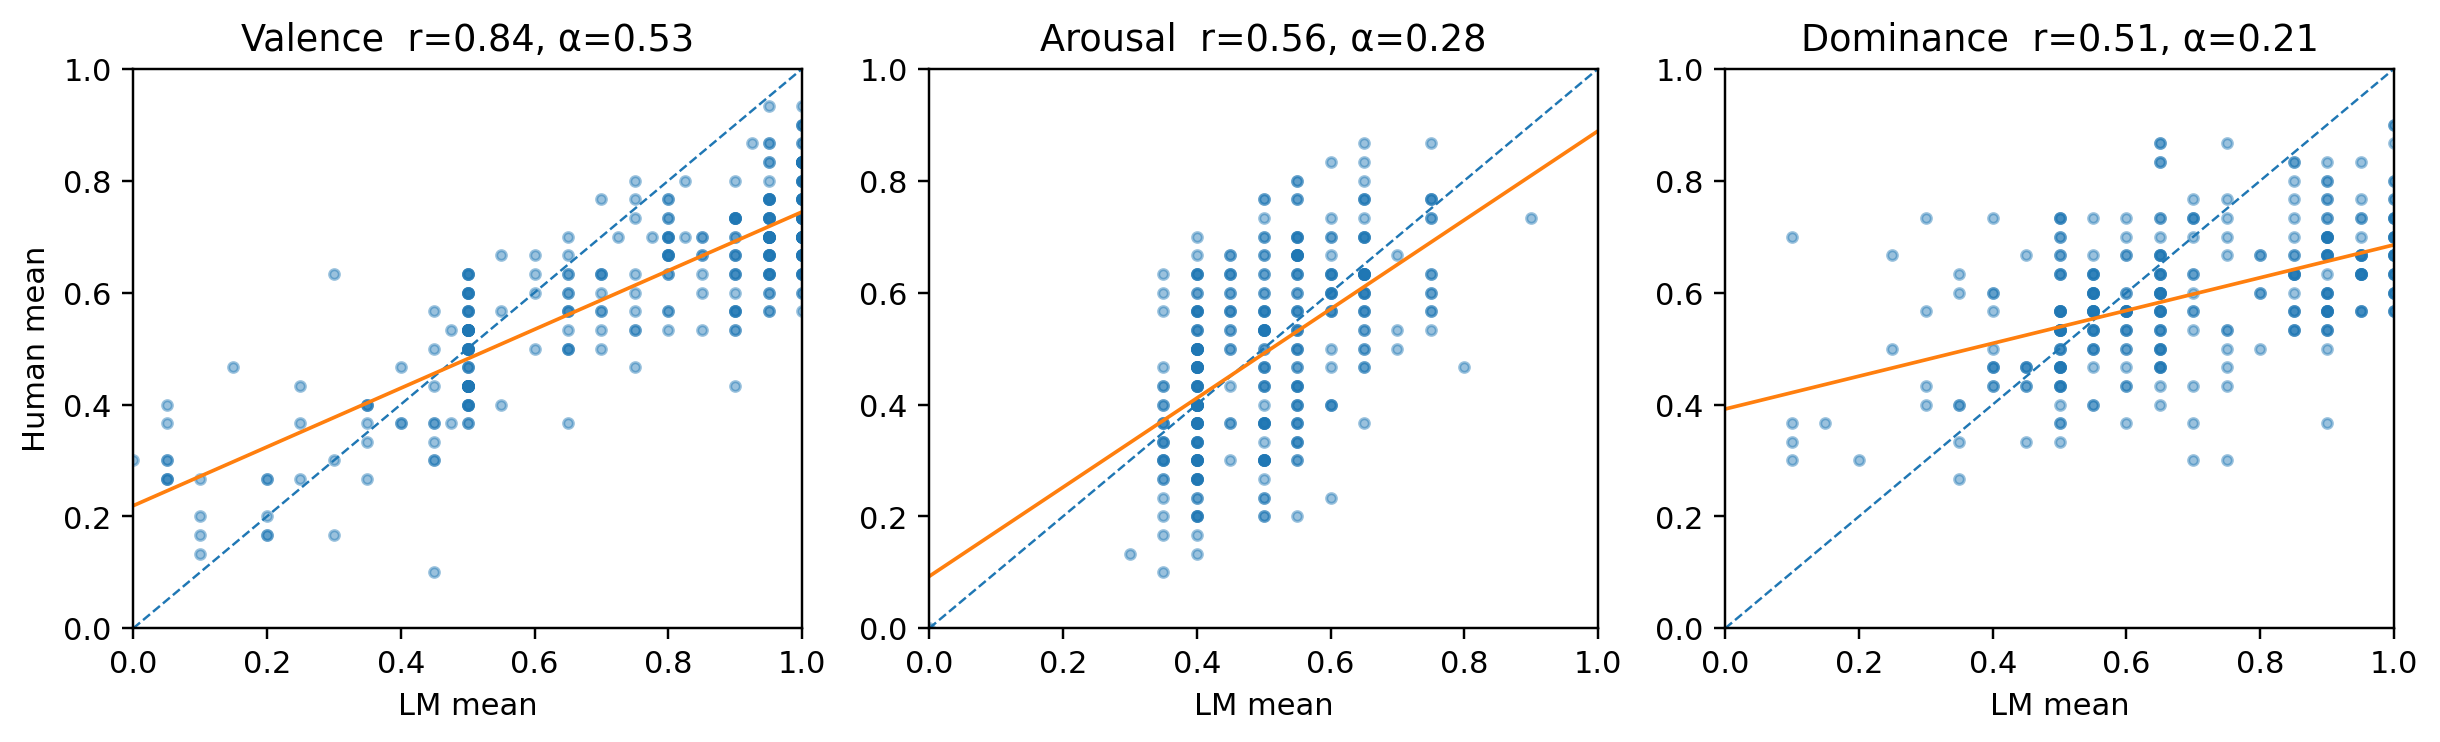
\includegraphics[width=0.96\textwidth]{figures/fig_human_validation.png}
\caption{Two-judge mean scores versus mean human scores for 300 items. Dashed
lines indicate perfect agreement and solid lines are least-squares fits; panel
titles report rounded Pearson $r$ and human Krippendorff $\alpha$.}
\label{fig:human-validation}
\end{figure}

\paragraph{Judge failure cases.}
Three audited items with $|\Delta|\geq 0.25$ show a common pattern: LM
judges latch onto evaluative surface markers rather than experiential force.
Importance markers inflate arousal; diplomatic framing inflates valence; a
crisis-framed political narrative suppresses dominance even when the event
described was a forcible seizure of power.

\paragraph{Score distributions and topic priors.}
On the eight-model subset, both judges produce unimodal distributions without clustering at round
values (no quantization). Hallucination-flagged generations show
$\Delta\text{Val}=-0.12$, $\Delta\text{Dom}=-0.09$,
confirming sensitivity to text content. Their agreement is strongest for
valence and weaker for arousal and dominance, so the full-panel analysis is
interpreted as conditional on the primary judge.

\section{Post-Hoc Clustering of 19 Models}
\label{sec:clustering}

We cluster all 19 models by a four-dimensional affective and response-behaviour profile
(mean Valence, Arousal, Dominance, and generic-answer rate) using Ward-linkage
hierarchical clustering on the Euclidean distance between profile vectors.
Models span diverse families, sizes (7B--27B), and capability tiers;
no origin labels are used at the clustering stage.

A note on interpretation: generic-answer rate is included as a clustering
feature, so the observation that clusters differ in generic-answer rate is
partly built into the construction.
The substantive claim is different: within each cluster, and after
excluding generic responses entirely, the arousal separation persists
($\Delta_{\text{arousal}} = -0.14$ between C1 and C3, $n=500$ targets),
showing that the cluster structure reflects genuine differences in
affective framing intensity, not only differences in how often models
deflect the prompt.

\paragraph{Cluster structure.}
Figure~\ref{fig:dend19} shows the dendrogram.
At a cut of $k=3$ clusters, the partition is:

\begin{itemize}
  \item \textbf{Cluster~1 (``Evasive''): YandexGPT, Ministral-8B, Qwen2.5-7B, Qwen2.5-Coder-14B.}
        Mean arousal $0.36$; generic-answer rate $30$--$55\%$.
        The defining feature is not origin but response behaviour: all four produce
        high rates of generic or templated output, which the judge consistently
        scores at low arousal.
  \item \textbf{Cluster~2 (``Moderate''): Qwen2.5-14B, AVIBE, Phi-3-Medium, Granite-4.1,
        Mistral-Nemo, SOLAR-10.7B, Llama-3-8B, Granite3.3-8B.}
        Mean arousal $0.41$; generic-answer rate $8$--$22\%$.
        The broadest cluster; models with average expressiveness and low
        refusal rates.
  \item \textbf{Cluster~3 (``Expressive''): Mistral-7B, GigaChat, Qwen3.6-27B,
        T-pro-it-2.1, Ministral-14B, Gemma-4-26B, GLM-4.7.}
        Mean arousal $0.53$; generic-answer rate $<12\%$.
        High-arousal expressive responses across all targets.
\end{itemize}

\begin{figure}[!htbp]
\centering
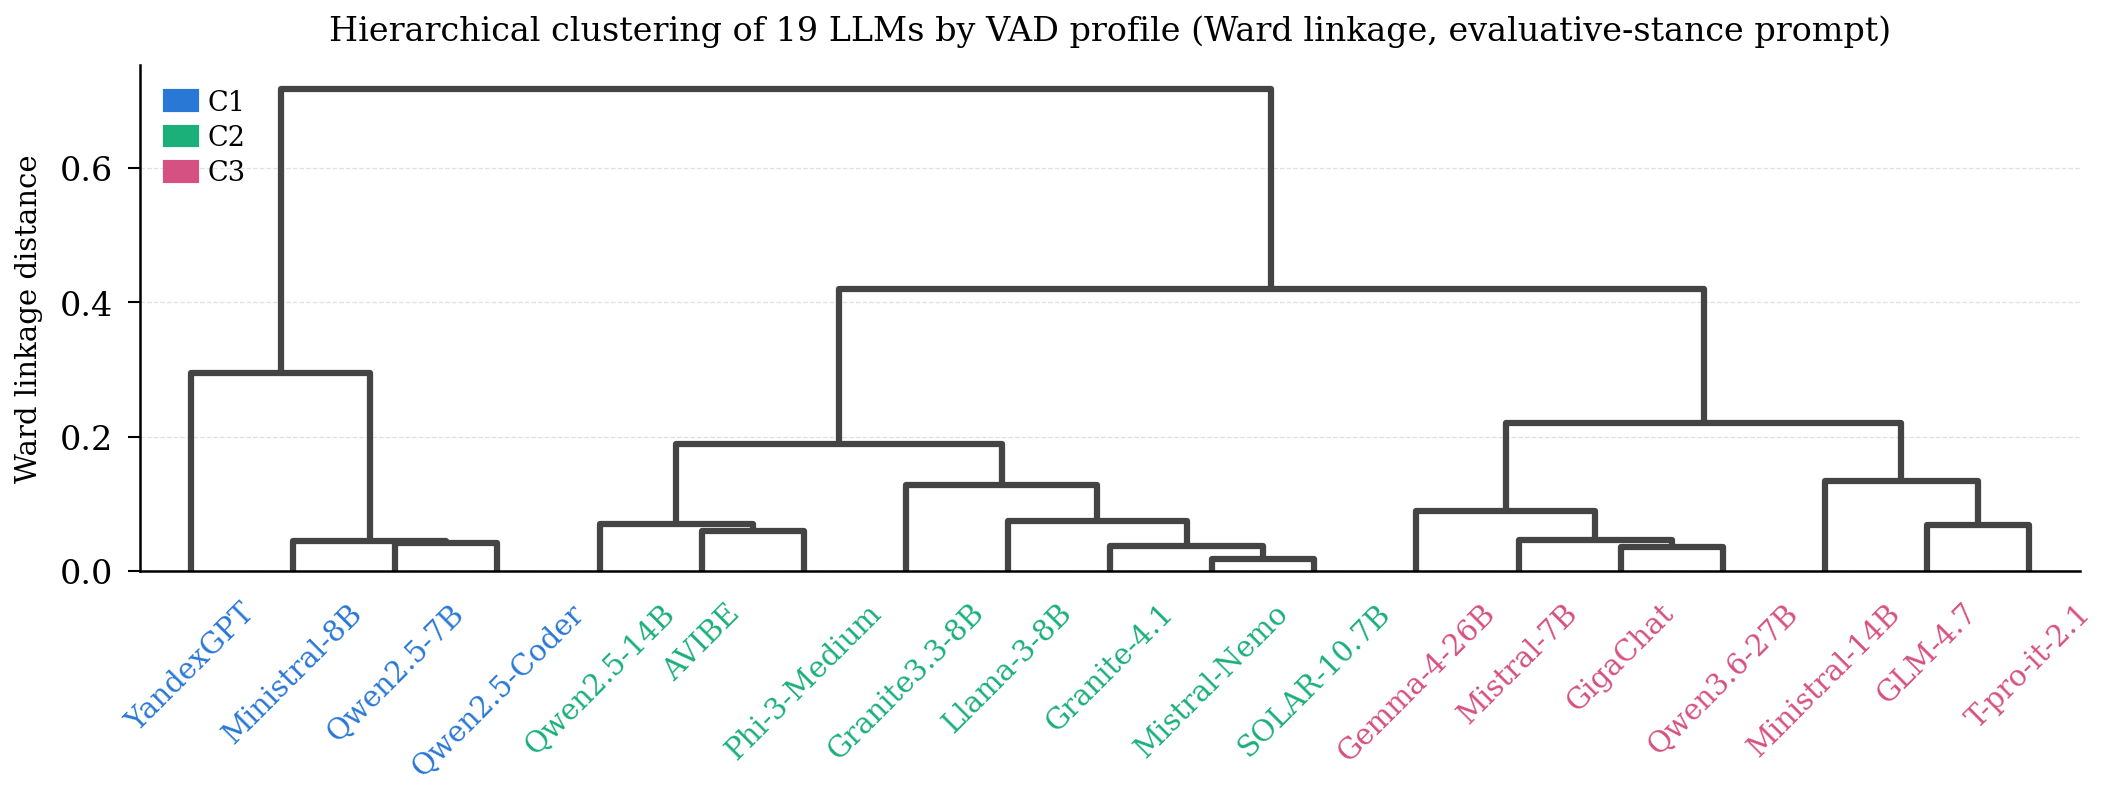
\includegraphics[width=\textwidth]{figures/fig_cluster_dendrogram_19.png}
\caption{Ward-linkage dendrogram over 19 LLMs clustered by mean affective and response-behaviour profile
(evaluative-stance prompt, $n=500$ targets, Qwen3.6-35B-A3B judge).
Leaf colours indicate cluster membership (blue = C1, green = C2, magenta = C3).}
\label{fig:dend19}
\end{figure}

\begin{figure}[!htbp]
\centering
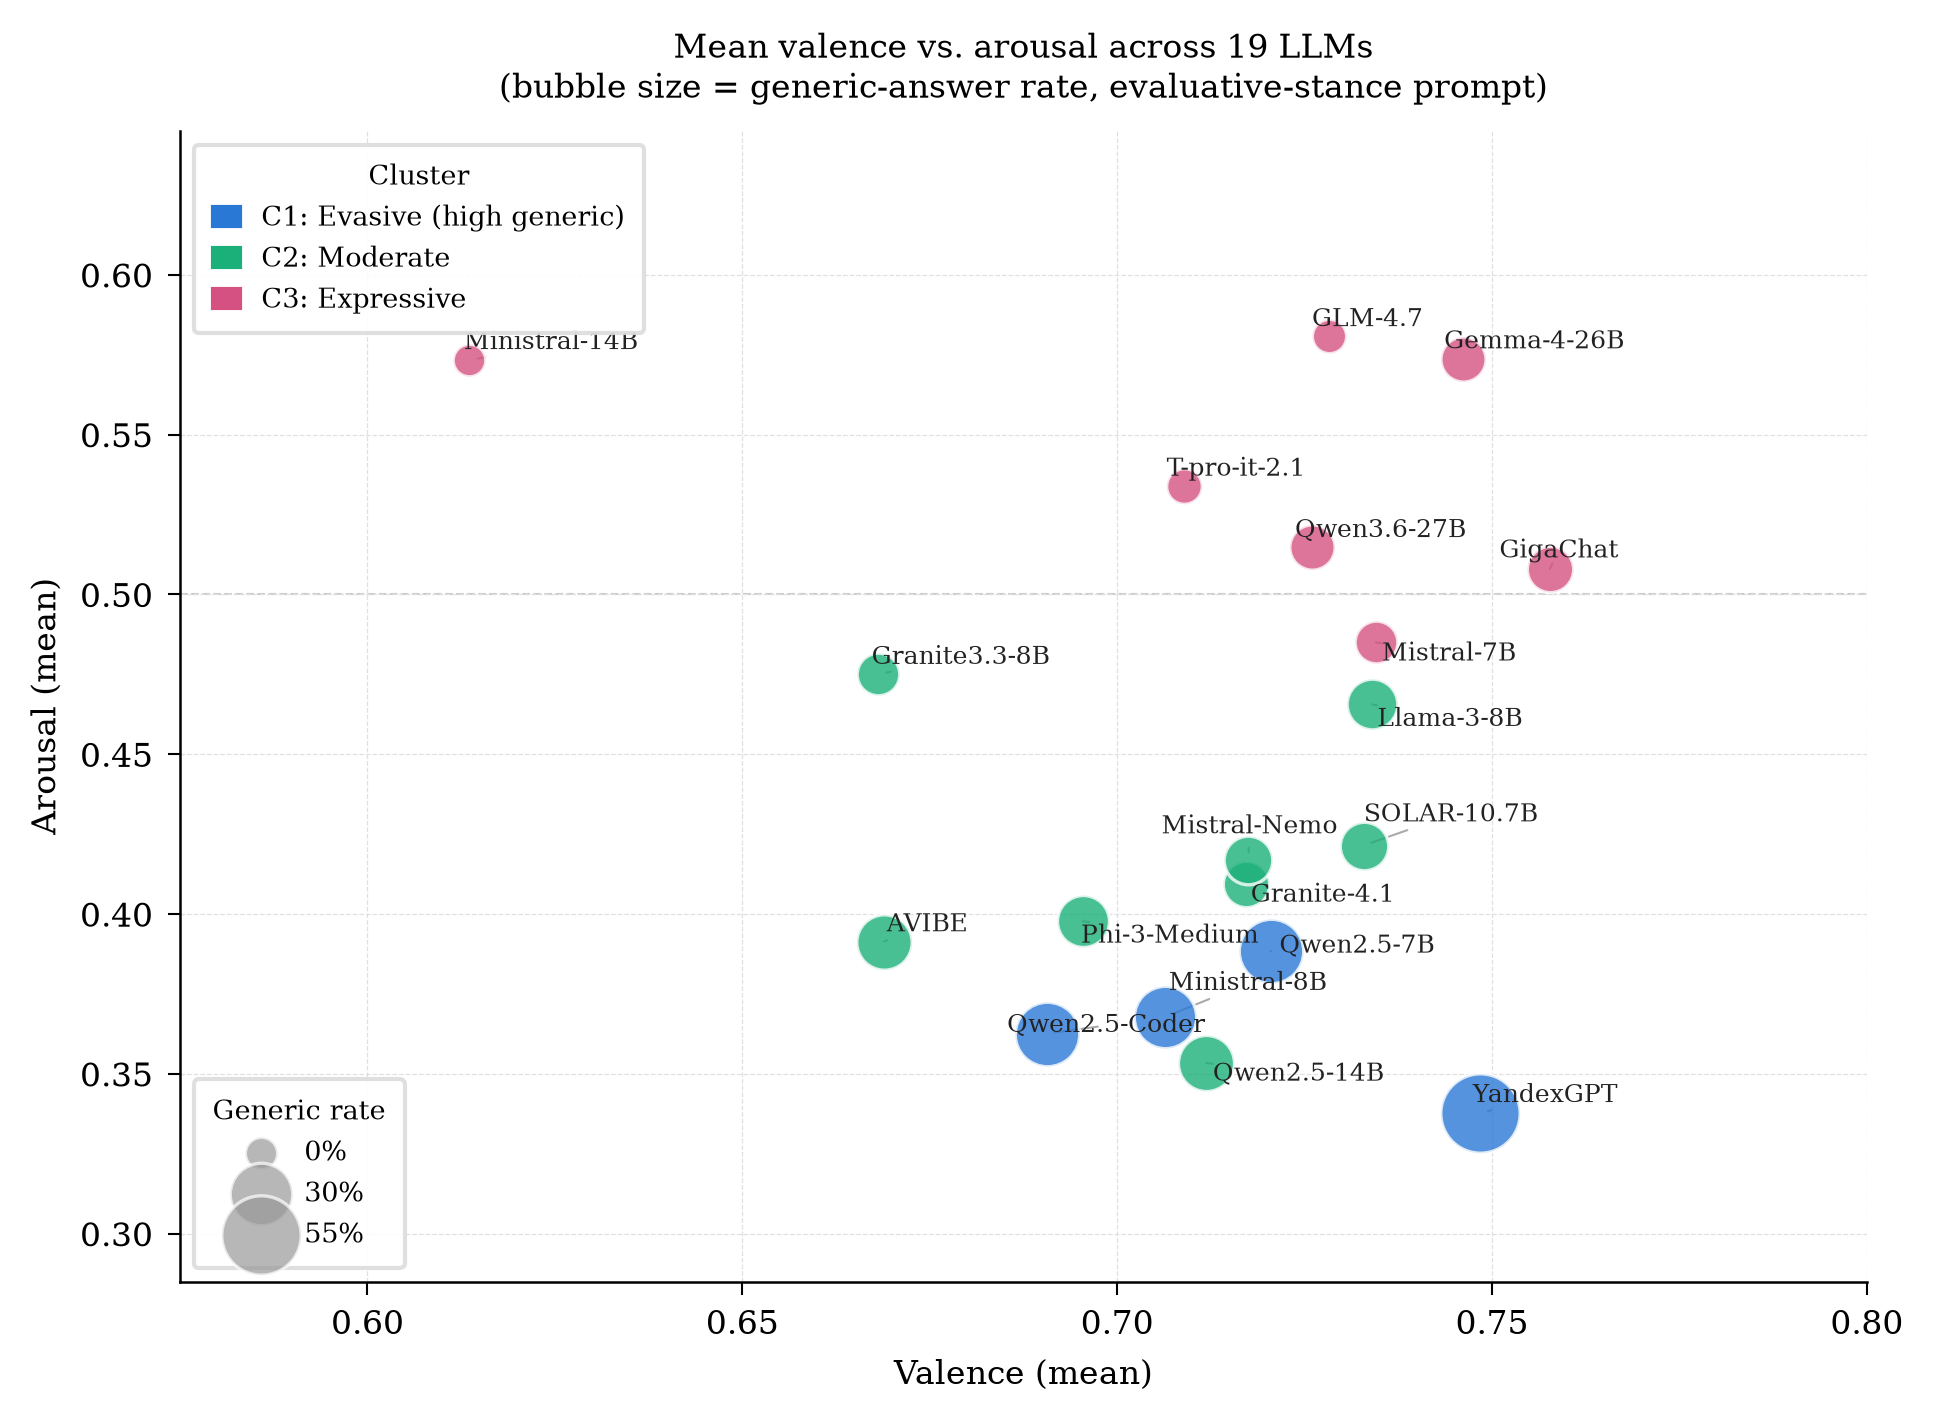
\includegraphics[width=0.75\textwidth]{figures/fig_cluster_scatter_19.png}
\caption{Mean valence vs.\ arousal across 19 LLMs (evaluative-stance prompt).
Bubble size encodes generic-answer rate. Colour indicates cluster.}
\label{fig:scatter19}
\end{figure}

\begin{figure}[!htbp]
\centering
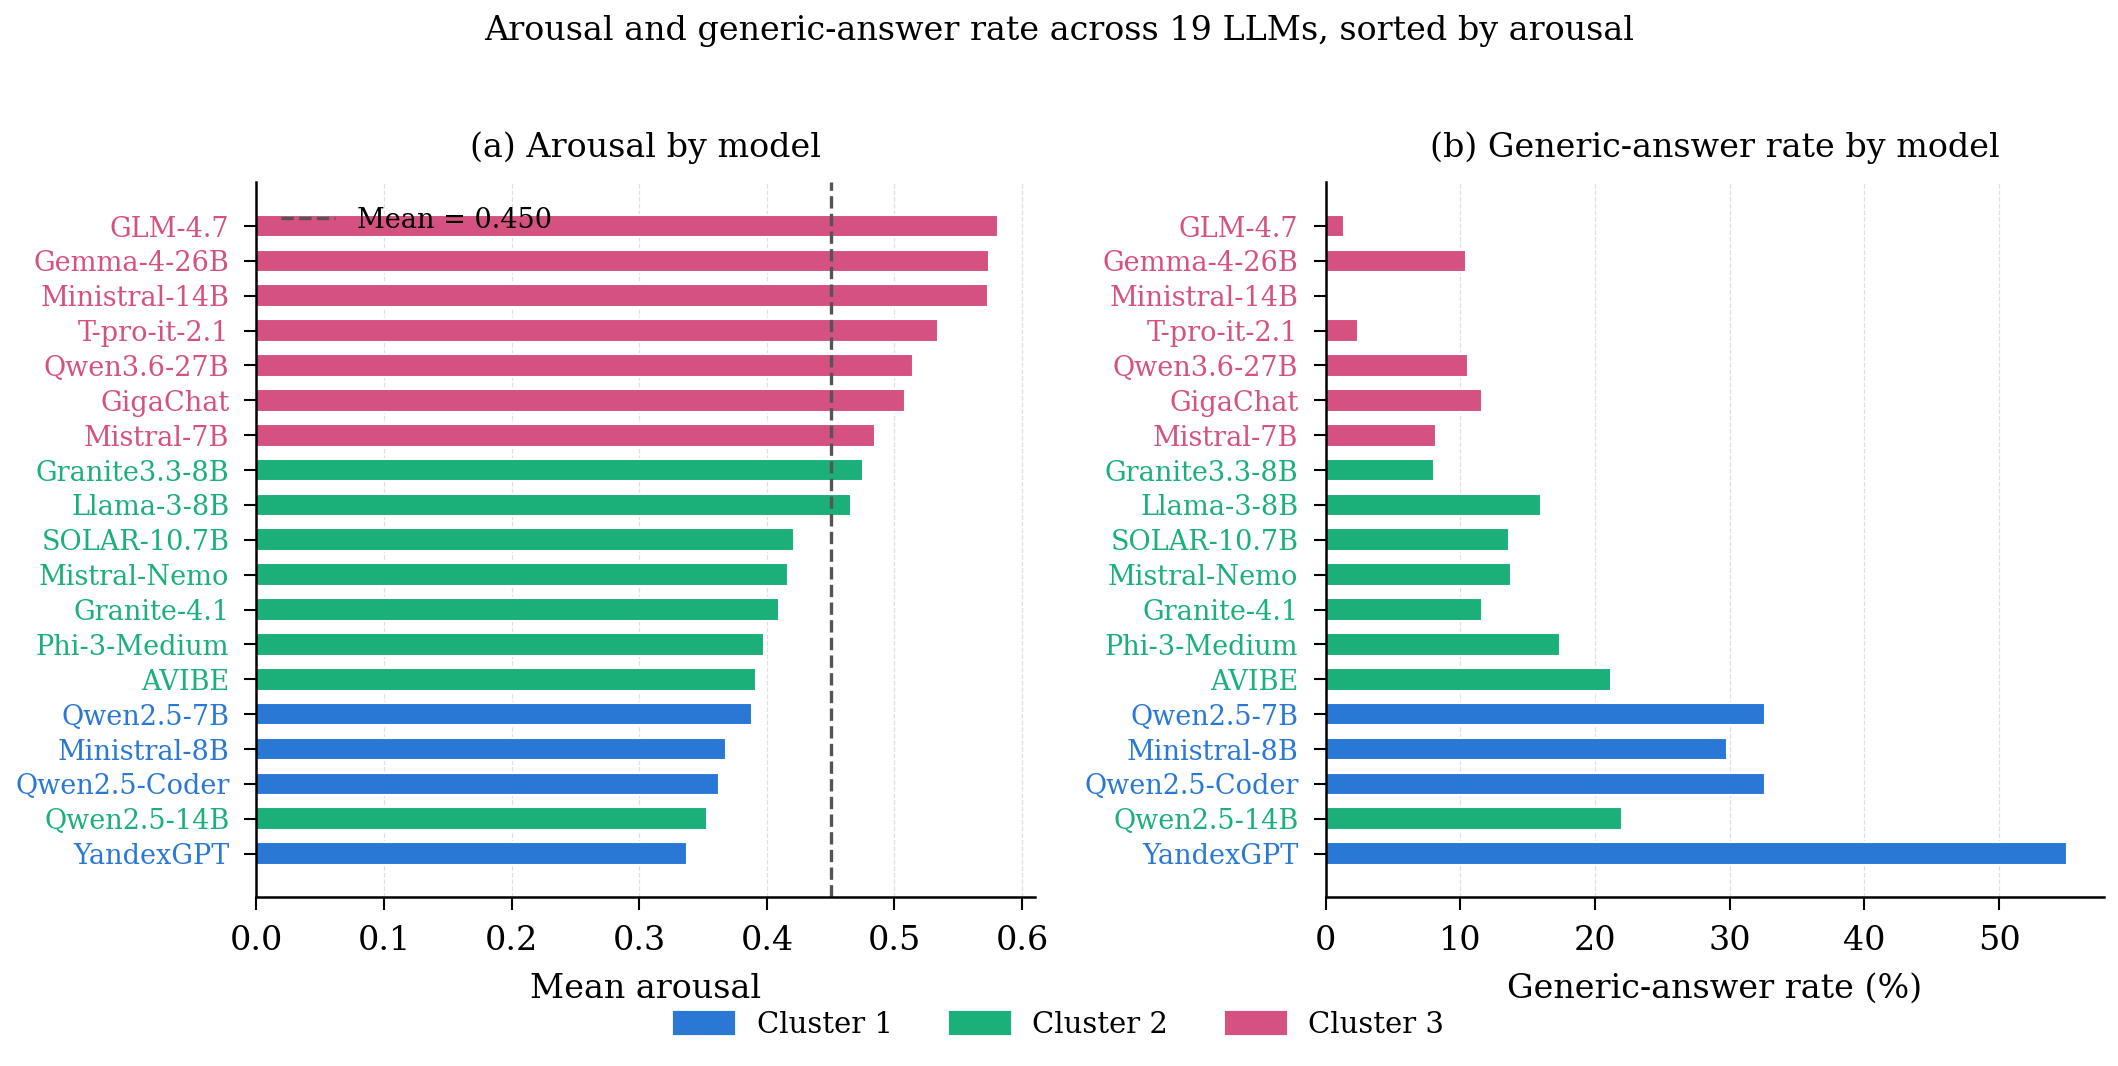
\includegraphics[width=\textwidth]{figures/fig_cluster_bars_19.png}
\caption{(a) Mean arousal and (b) generic-answer rate across 19 LLMs, sorted
by arousal. Colour indicates cluster.}
\label{fig:bars19}
\end{figure}

\paragraph{Key observations.}
First, the cluster partition does not reproduce the Russian-developed/non-Russian split.
GigaChat and T-pro-it-2.1 (Russian-developed) land in the high-arousal Cluster~3
alongside GLM, Gemma, and Mistral families.
YandexGPT (Russian-developed) is grouped with Ministral-8B, Qwen2.5-7B, and
Qwen2.5-Coder-14B in Cluster~1 --- models that, despite different origins,
share a tendency to produce evasive, generic-phrased responses under the evaluative prompt.
AVIBE (Russian-developed) joins the moderate Cluster~2.

Second, the primary axis of variation across models is \emph{arousal},
with generic-answer rate as a confounding moderator.
Arousal spans from $0.34$ (YandexGPT) to $0.58$ (GLM),
while valence stays in a narrow band ($0.61$--$0.76$) with no systematic
cluster ordering (Figure~\ref{fig:scatter19}).

Third, YandexGPT's low arousal is largely attributable to its high
generic-answer rate ($55\%$), as the judge assigns low arousal to
templated non-committal responses. The cluster analysis shows this is not
a property specific to Russian-developed models: Qwen2.5-7B and
Qwen2.5-Coder-14B, despite different origins, land in the same evasive
cluster for the same reason.

\paragraph{Additional findings.}
Beyond the cluster structure itself, the expanded panel reveals three further patterns.

\textbf{Arousal and generic-answer rate are tightly coupled across all 19 models.}
The Pearson correlation between mean arousal and generic-answer rate is
$r = {-0.81}$ ($p < 0.001$, $n = 19$; 95\% bootstrap CI $[-0.91,\,-0.71]$).
This is not a within-cluster artifact: the relationship holds globally, spanning
the full range from GLM ($A = 0.58$, generic $= 1\%$) to YandexGPT ($A = 0.34$, generic $= 55\%$).
The evaluative-stance prompt appears to trigger either committed framing
(low generic, high arousal) or templated deflection (high generic, low arousal),
with few models occupying a middle ground on both dimensions simultaneously.

\textbf{Dominance varies across clusters in the same direction as arousal.}
Cluster~3 (expressive) shows the highest mean dominance ($0.694$),
followed by Cluster~2 (moderate, $0.670$) and Cluster~1 (evasive, $0.651$),
a gradient of $+0.043$ units from C1 to C3.
Valence, by contrast, is nearly flat across clusters
(C1: $0.719$, C2: $0.706$, C3: $0.724$) --- a C3$-$C1 difference of only $+0.005$.
Cross-model correlations qualify this cluster-level pattern: arousal and dominance
are moderately associated ($r = 0.46$ across 19 models), while arousal and valence
are essentially unrelated ($r = -0.05$).
Generic-answer rate is strongly associated with arousal ($r = -0.80$), moderately
associated with dominance ($r = -0.41$), and only weakly associated with valence
($r = +0.24$; not significant).
The cluster-level arousal--dominance co-movement suggests that when a model avoids committing
to a stance, it simultaneously reduces both the intensity and the assertiveness of
its output, while the positive--negative register remains unchanged.

\textbf{Model family does not predict cluster.}
The Qwen2.5 family splits across all three clusters:
Qwen2.5-Coder-14B and Qwen2.5-7B are evasive (C1), Qwen2.5-14B is moderate (C2),
and Qwen3.6-27B is expressive (C3).
Similarly, the two Granite models land in C2 despite architectural similarity.
This suggests that instruction-tuning decisions --- specifically how the model
handles evaluative or politically adjacent prompts --- matter more for affective
output than base architecture or parameter count.

\paragraph{Cluster differences by target category.}
Figure~\ref{fig:cat-vad} shows all three VAD axes broken down by category and cluster.
The axes tell strikingly different stories.

\emph{Arousal} is the only axis with a consistent, large C3$-$C1 gap across all six
categories (range $+0.123$ to $+0.225$).
Cultural objects and places show the largest separation ($+0.225$):
expressive models respond to monuments, traditions, and UNESCO-listed sites with
substantially higher emotional intensity than evasive ones.
Persons and countries follow closely ($+0.211$ and $+0.192$), while organisations
and social groups show the smallest gap ($+0.123$ and $+0.127$) --- these targets
are framed institutionally rather than emotionally.

\emph{Valence} shows no such ordering: the C3$-$C1 gap is near zero or weakly
negative for persons ($-0.039$), events ($-0.039$), countries ($-0.027$), and
organisations ($-0.025$), with only cultural symbols showing a modest positive gap
($+0.067$).
Expressive models do not assign higher positive sentiment; they assign higher intensity.

\emph{Dominance} follows arousal in direction but with much smaller magnitude
(range $-0.013$ to $+0.099$): cultural symbols again show the largest gap ($+0.099$),
while events are near zero ($-0.013$).

\begin{figure}[!htbp]
\centering
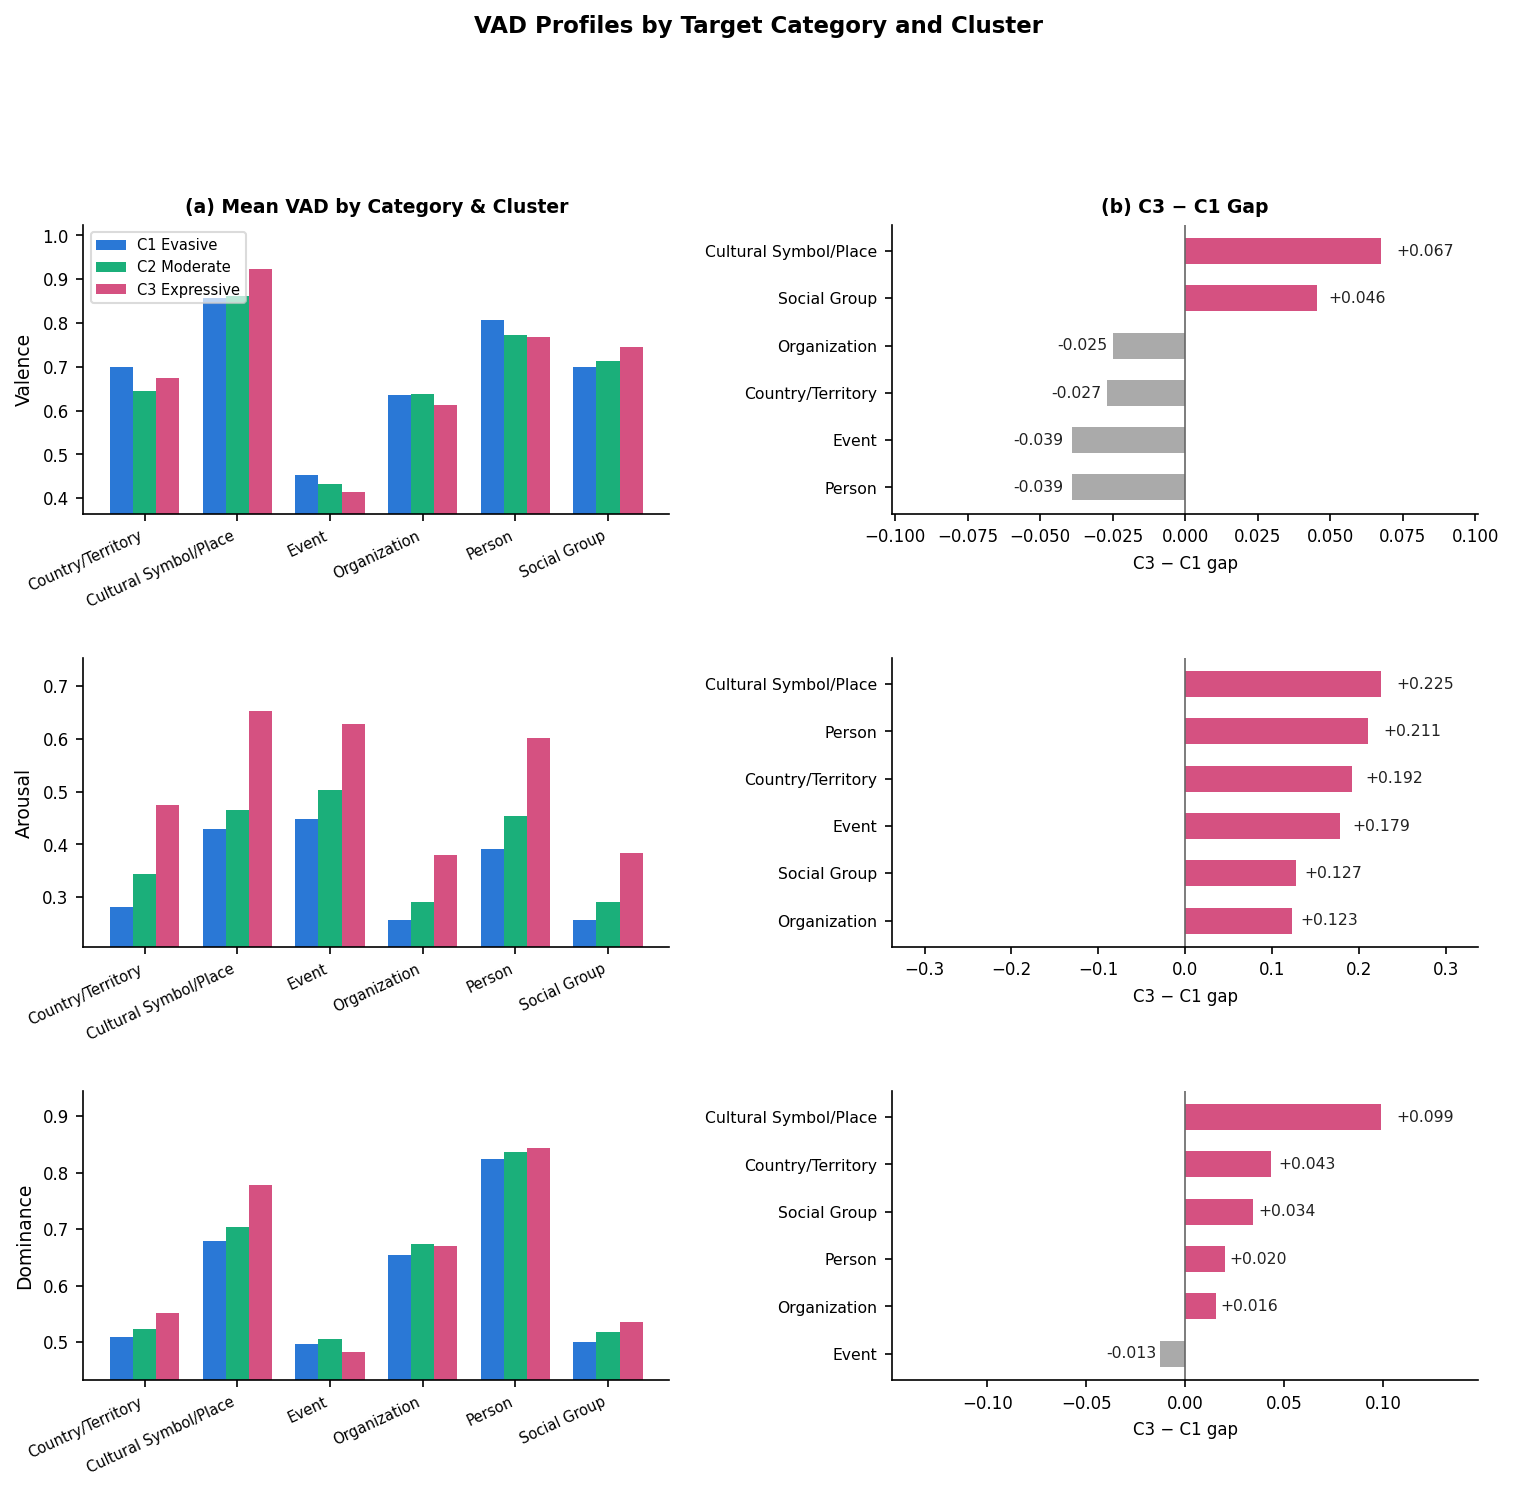
\includegraphics[width=\textwidth]{figures/fig_category_vad.png}
\caption{Mean Valence, Arousal, and Dominance by target category and cluster
(evaluative-stance prompt, 19 models, Qwen3.6-35B-A3B judge).
Left column: grouped bars per cluster. Right column: C3$-$C1 gap.
Arousal shows a large, consistent gap across all categories; valence shows
near-zero or negative gaps; dominance follows arousal at reduced magnitude.}
\label{fig:cat-vad}
\end{figure}

\paragraph{Cluster separation by country.}
The country-level breakdown shows the same three-axis pattern.

\emph{Arousal} gaps are large and positive for every country (range $+0.156$ to
$+0.217$): Georgia ($+0.217$), Armenia ($+0.216$), and Ukraine ($+0.206$) show the
largest separation; Turkmenistan ($+0.156$) and Uzbekistan ($+0.157$) the smallest.
The countries with the largest cluster gap are precisely those with high geopolitical
salience and contested representation --- Georgia (2008 war), Armenia
(Nagorno-Karabakh), Ukraine (ongoing conflict).

\emph{Valence} gaps are small and mixed: roughly half the countries show positive
gaps and half negative (range $-0.052$ to $+0.036$), with no pattern matching the
arousal ranking.
Russia, Ukraine, and Georgia --- the three most politically salient countries ---
occupy opposite ends of the valence gap ranking, confirming that valence does not
track contestedness.

\emph{Dominance} gaps are consistently positive but modest (range $+0.007$ to
$+0.076$): Armenia ($+0.076$) and Georgia ($+0.072$) lead, echoing the arousal
pattern at roughly one-third the magnitude.
Russia stands out on absolute dominance level
(C1: $0.777$, C3: $0.804$) --- substantially higher than any other country ---
reflecting the large share of high-agency persons and institutions among Russian
targets.

\paragraph{Interpretation.}
The full VAD breakdown converges on a single conclusion: the cluster structure is
carried by arousal and, secondarily, by dominance.
Valence --- the axis captured by conventional sentiment analysis --- is flat across
clusters, countries, and categories alike ($r(\text{generic}, V) = +0.24$, not
significant).
Models that deflect evaluative prompts do not produce more negative sentiment; they
produce \emph{less intense} framing.
This distinction is invisible to sentiment-only measurement but directly observable
in the arousal and dominance axes of the VAD framework.

\section{Discussion}
\label{sec:discussion}

\paragraph{Generic-answer rate as the strongest correlate.}
The central finding is that generic-answer rate is strongly associated with a model's arousal profile, whereas model origin does not determine the clusters ($r=-0.81$ across 19 models).
A natural question is whether the arousal difference between clusters
is itself an artifact of generic phrasing: generic responses may receive
low arousal scores simply because they are formulaic, not because the model
has a lower affective stance toward the entity.
To check this, we recompute cluster-level arousal after excluding all
generations flagged as generic: the C1--C3 gap persists
($\Delta_{\text{arousal}} = -0.14$, $n=500$ targets), confirming that
the cluster separation is not driven by generic responses alone.
The arousal difference is present even within non-generic outputs.

\paragraph{Knowledge gap alternative.}
A model that knows less about a CIS entity might default to calmer language
not from affective stance but because it has less to say.
Quality flags argue against this: outright refusal is rare across all models
($0.2\%$--$0.5\%$), and target coverage is high and comparable across clusters.
The Spitak earthquake example is illustrative:
YandexGPT (C1) produces a substantive, on-topic response --- it is not
failing to recognise the target --- yet frames the same event at arousal~$0.60$
while Gemma-4-26B (C3) reaches arousal~$0.95$.
The difference is in framing intensity, not in knowledge coverage.

\paragraph{What VAD surfaces that sentiment does not.}
Both Spitak-earthquake responses are negative in valence.
A sentiment classifier would treat them as equivalent.
VAD profiling separates them on arousal --- calm acknowledgement vs.\
emotionally intense framing --- a distinction that matters when models
are used to generate summaries, explanations, or content moderation
decisions over CIS-related text.
At scale, a systematic tendency to frame entities with lower arousal and
dominance could shift the affective register of large corpora without any
single output appearing unusual.
Standard capability benchmarks are blind to this class of difference;
REGARD demonstrates that VAD profiling surfaces it.

\paragraph{Instruction tuning rather than origin.}
The cluster analysis shows that the Qwen2.5 family splits across all three
clusters, and the two Russian-developed models with the lowest generic rates
(GigaChat, T-pro-it-2.1) land in the expressive cluster alongside GLM and
Gemma.
This pattern makes instruction-tuning decisions --- specifically, how a model
is trained to respond to evaluative prompts about politically adjacent
entities --- one plausible mechanism for the arousal variation. It does not
support attributing the variation to a shared property of Russian-developed
models as a class.

\section{Limitations}
\label{sec:limitations}

\paragraph{Exploratory status.}
The study was not preregistered: the Ward clustering and the emphasis on
arousal followed inspection of the score profiles. They should therefore be
read as exploratory structure in this finite model panel, not as confirmatory
population-level inference.

\paragraph{Cluster count.}
The number of clusters was set to $k=3$ by visual inspection of the
Ward-linkage dendrogram (Figure~\ref{fig:dend19}): the tree shows three
clearly separated subtrees at a linkage distance of approximately $0.30$,
with a large gap before the next merge.
All 19 models are analysed; no origin labels are used at the clustering
stage.

\paragraph{Prompt sensitivity.}
Results are reported on the evaluative-stance prompt.
Under a neutral-descriptive formulation the cluster separation in arousal
narrows but remains present; under an evaluative paraphrase it weakens
further. The finding that arousal is the primary axis of variation is
specific to prompts that invite an evaluative stance; it may not generalise
to purely descriptive or factual generation settings.

\paragraph{Generation variance.}
Each model--target--prompt condition contains one stochastic generation at
temperature~$0.7$. Consequently, the study cannot estimate within-model
sampling variance; repeated generations are needed to separate stable
model behaviour from decoding variability.

\paragraph{Arousal measurement.}
On the eight-model subset, judge-vs-judge agreement on arousal is lower than
on valence ($r=0.460$ vs.\ $r=0.885$), reflecting the inherent subjectivity
of intensity judgements. Human validation yields $r=0.565$, above the noise
floor but below the valence benchmark. The other 11 models do not have
second-judge or human validation, so absolute arousal values and the resulting
full-panel cluster structure should be interpreted as conditional on the
primary Qwen judge.

\paragraph{Language confound.}
All generations are elicited in Russian. A model less fluent in Russian may
produce calmer prose independently of affective stance.
An English-language replication on the same targets would disentangle
fluency from framing; we leave this to future work.

\paragraph{Scope of ``Russian-developed.''}
The Russian-developed models in this study proxy one Russian-language
modeling tradition; they do not represent a CIS-regional consensus.
Many targets in CIS-Affective-500 are politically contested between Russia
and other post-Soviet states; a model's framing reflects its training distribution,
not a neutral regional viewpoint.
Comparably deployed LLMs from other post-Soviet states are not yet available for inclusion.

\paragraph{Judge priors.}
Both automated judges are non-CIS models; on the validation subset, any shared
affective framing of post-Soviet entities may systematically diverge from
CIS-audience perception. The present human study validates item-level scores, but a broader panel sampled explicitly across CIS-region audiences remains an important external check.


\section{Conclusion}
\label{sec:conclusion}

We presented REGARD, an empirical study of affective framing in LLMs
on CIS-related entities, using a curated bank of 500 targets, 19 generator
models, and a primary VAD judge with independent second-judge and human
validation on an eight-model subset.

Post-hoc Ward-linkage clustering of all 19 models by affective and response-behaviour profile reveals
three behavioural clusters --- Evasive, Moderate, and Expressive ---
that cut across model origin, family, and parameter count.
Generic-answer rate is strongly associated with lower arousal ($r = -0.81$) and with cluster placement, whereas regional origin does not determine the clusters: models that deflect
evaluative prompts with templated responses cluster together at low arousal
regardless of where they were developed.
The arousal gap is largest for culturally and politically salient targets
(persons, cultural objects, countries) and smallest for institutional ones
(organizations, social groups).
The cluster separation survives exclusion of generic responses, while the
subset validation shows that arousal is less reliably measured than valence.
VAD profiling surfaces a dimension of model behaviour --- emotional
intensity of framing --- that is invisible to sentiment-only measurement
and not captured by standard capability benchmarks.

\section*{Data and Code Availability}
Code, paper sources, and data-access instructions are available at
\url{https://github.com/ikanam-ai/MEGA/tree/main/REGARD}.

\FloatBarrier
\begin{credits}
\subsubsection{\ackname}
This work was supported by a grant provided by the Ministry of Economic
Development of the Russian Federation in accordance with the subsidy agreement
(agreement identifier 000000C313925P4G0002) and the agreement with the Ivannikov
Institute for System Programming of the Russian Academy of Sciences dated
June 20, 2025, No. 139-15-2025-011. The authors thank Nikolai Stukalov for his
contribution to data annotation.

\subsubsection{\discintname}
The authors have no competing interests to declare that are relevant to the
content of this article.
\end{credits}

\bibliographystyle{splncs04}
\bibliography{main}
\end{document}
